\chapter{Introducción}
\label{cap:introduccion}


\section{Contexto}

Las redes Peer-to-Peer (P2P) representan un modelo de comunicación descentralizado en el que todos los nodos participan de forma equitativa, actuando tanto como clientes como servidores.
Este paradigma, alternativo al modelo cliente-servidor tradicional, ha transformado la forma en que compartimos información y utilizamos los recursos en línea.
Su impacto ha sido especialmente notable en el ámbito del intercambio de archivos, donde su capacidad para distribuir grandes volúmenes de datos sin depender de servidores centralizados ha supuesto una revolución tecnológica \cite{schollmeier2001}.

\begin{figure}[h]
    \centering
    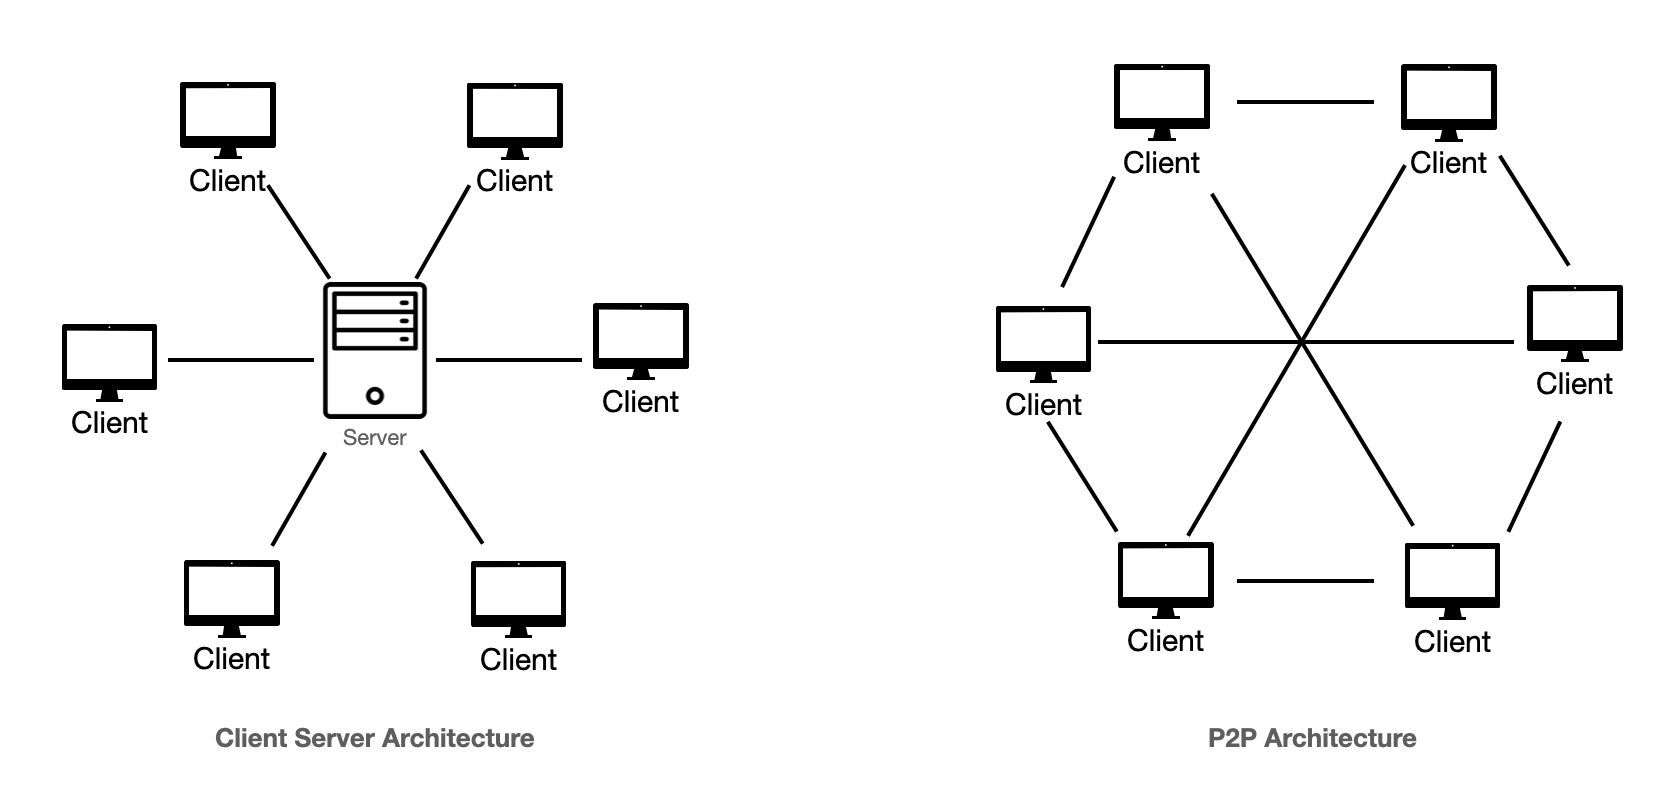
\includegraphics[width = 0.5\textwidth]{Imagenes/Vectorial/client-server-vs-p2p}
    \caption{Comparaci\'on entre arquitectura cliente-servidor y arquitectura P2P}
    \label{fig:clientVsp2p}
\end{figure}


Las redes P2P no solo destacan por su arquitectura innovadora, sino también por su impacto en la democratización del acceso a los recursos digitales.
Al eliminar la necesidad de intermediarios centralizados, estas redes permiten a los usuarios compartir directamente recursos como archivos, ancho de banda o poder computacional.
Esto ha impulsado aplicaciones clave en dominios que van desde el intercambio de contenido multimedia hasta la computación distribuida.

Sin embargo, este modelo también plantea retos significativos.
La ausencia de un punto central de control introduce la necesidad de desarrollar mecanismos eficientes para la localización de recursos, la gestión del tráfico de red y la seguridad de las comunicaciones.
Estos desafíos han impulsado avances tecnológicos en áreas como el diseño de algoritmos distribuidos y la optimización de protocolos de comunicación.

En la actualidad, las redes P2P son fundamentales en aplicaciones que requieren escalabilidad y descentralización.
Desde servicios de streaming y distribución de videojuegos hasta sistemas basados en blockchain como Bitcoin,
estas tecnologías representan un cambio hacia infraestructuras digitales más resilientes.
Más allá de su uso técnico, las redes P2P simbolizan un paradigma donde el control se distribuye, empoderando a los usuarios finales.



\section{Motivación}

Las redes Peer-to-Peer (P2P) han transformado la manera en que compartimos información y utilizamos recursos en línea,
posicionándose como una alternativa eficiente y escalable al modelo cliente-servidor.
A pesar de su relevancia y aplicaciones actuales en campos como el intercambio de archivos, el streaming de vídeo y las plataformas blockchain,
el diseño e implementación de estas redes desde un nivel práctico sigue siendo un reto para muchos desarrolladores.

Este trabajo no busca competir con las grandes plataformas que emplean arquitecturas P2P ni desarrollar una red masiva con millones de usuarios.
En cambio, se enfoca en la creación de una red P2P funcional desde cero, con énfasis en los conceptos fundamentales y su implementación práctica.

Con ello, se espera facilitar el entendimiento de este modelo descentralizado y motivar el desarrollo de nuevas aplicaciones basadas en redes P2P,
adaptadas a los desafíos tecnológicos contemporáneos.


\section{Objetivos}

El objetivo principal de este trabajo es diseñar e implementar una red Peer-to-Peer (P2P) funcional para el intercambio de archivos de manera distribuida,
integrando tecnologías actuales como UPnP para la gestión automática de puertos y un sistema centralizado para la localización y conexión de nodos.
Este desarrollo se centrará en la creación de un cliente con interfaz gráfica que sirva como base para todas las funcionalidades de la red.

Para alcanzar este objetivo general, se plantean los siguientes objetivos específicos:

\begin{itemize}
    \item \textbf{Desarrollar un cliente con interfaz gráfica:} Diseñar e implementar una aplicación gráfica que permita a los usuarios compartir y descargar archivos de manera sencilla e intuitiva. Este cliente será el núcleo sobre el cual se integrarán las funcionalidades de la red P2P.

    \item \textbf{Desarrollar un sistema de registro y gestión de nodos:} Implementar un mecanismo centralizado que permita identificar y coordinar los peers conectados a la red, facilitando su interacción y comunicación.

    \item \textbf{Diseñar e implementar la comunicación directa entre nodos:} Crear un protocolo basado en TCP que permita a los peers establecer conexiones fiables y seguras para el intercambio de archivos, asegurando una comunicación robusta y compatible con redes distribuidas.

    \item \textbf{Integrar soporte para UPnP:} Automatizar la configuración de puertos en los routers mediante el uso de UPnP, garantizando una conectividad sencilla y accesible para los usuarios.

    \item \textbf{Implementar un sistema de intercambio de archivos distribuido:} Diseñar un modelo que permita a los peers compartir y descargar archivos fragmentados desde múltiples fuentes, optimizando el uso de los recursos de la red.

    \item \textbf{Documentar el diseño, implementación y evaluación del sistema:} Elaborar una descripción técnica detallada del desarrollo de la red P2P, incluyendo los algoritmos y tecnologías utilizadas, así como las

\end{itemize}


\section{Plan de trabajo}

Durante el desarrollo del proyecto se ha seguido un plan de trabajo detallado con el objetivo de estructurar las tareas y garantizar el cumplimiento de los objetivos planteados. La planificación ha permitido organizar de forma eficiente las distintas fases del desarrollo, estableciendo prioridades y tiempos. El plan de trabajo se ha dividido en los siguientes puntos:

\begin{enumerate}

    \item \textbf{Estudio de las tecnologías a utilizar:}
    Se llevó a cabo un análisis detallado de las tecnologías necesarias para el desarrollo del proyecto, incluyendo protocolos de comunicación como TCP,
    sistemas de apertura de puertos con UPnP y arquitecturas P2P para el intercambio de archivos.
    Este estudio incluyó la búsqueda de documentación técnica, recursos en línea y herramientas que facilitaran el desarrollo.

    \item \textbf{Desarrollo del cliente con interfaz gráfica:}
    Se inició el diseño e implementación en java del cliente gráfico como base del proyecto.
    Este cliente incluye funcionalidades esenciales para compartir y descargar archivos, sirviendo como núcleo sobre el cual se desarrollaron las demás características de la red.
    Durante esta fase, se probaron aspectos básicos de la interacción con el sistema de archivos local.

    \item \textbf{Implementación del sistema de registro de nodos:}
    Se diseñó e implementó un sistema centralizado para gestionar los nodos conectados a la red.
    Este sistema permite registrar los peers activos y facilitar su descubrimiento entre ellos.
    Además, se integró con el cliente para garantizar que los usuarios pudieran conectarse a otros peers de manera eficiente.

    \item \textbf{Diseño e implementación de la comunicación entre nodos:}
    Se desarrolló un protocolo basado en TCP para la conexión directa entre peers.
    Esta etapa incluyó pruebas para garantizar la fiabilidad y estabilidad de las conexiones, así como su integración con el cliente gráfico.

    \item \textbf{Integración del soporte para UPnP:}
    Se implementó soporte para la configuración automática de puertos mediante UPnP, lo que permitió facilitar la conexión entre nodos en redes con configuraciones complejas,
    eliminando la necesidad de ajustes manuales por parte del usuario.

    \item \textbf{Evaluación y pruebas del sistema:}
    Se llevaron a cabo pruebas funcionales para verificar el correcto funcionamiento de cada componente de la red P2P, así como su integración global.
    Estas pruebas incluyeron casos con múltiples nodos conectados para garantizar la robustez del sistema.

    \item \textbf{Escritura y revisión de la memoria:}
    Durante las fases de implementación y pruebas, se elaboró la memoria del proyecto, documentando las decisiones tomadas, los resultados obtenidos y los aprendizajes adquiridos.

    \item \textbf{Cierre del proyecto:}
    Una vez terminadas todas las fases, se realizó una revisión final del cliente y de la memoria, realizando las correcciones necesarias para su entrega final.
    Se verificó que todos los objetivos se hubieran cumplido satisfactoriamente antes del cierre del proyecto.
\end{enumerate}

En definitiva, un plan de trabajo bien estructurado ha permitido avanzar de manera eficiente y cumplir con los hitos establecidos dentro del tiempo límite.

\section{Organizaci\'on de la memoria}